\usetikzlibrary{shapes.callouts}
\lstset{basicstyle=\ttfamily,language=C}
\begin{document}
\title{Übungsblatt~7}
\subtitle{Pufferverwaltung}
\maketitle

\section*{Lernziele}
\begin{itemize}
	\item Notwendigkeit und Arbeitsweise des Datenbankpuffers
	\item Verwendung von Schnittstellen in der Schichtenarchitektur
\end{itemize}

\begin{normalText}
\section*{Literatur}
\HaerderNintyNine{5}

\ElmasriFive{14}

\BovetThird{17.3}
\end{normalText}

\section*{Links}
\begin{description}
	\ViseAuD
\end{description}


\section{Fragen zur Vorlesung}
\begin{enumerate}[a)]
	\item Wozu dient der Datenbankpuffer?

	\begin{solution}
	Der Datenbankpuffer dient dem Zwischenspeichern von Daten im Hauptspeicher. Ziel ist es, die Performance zu erhöhen, indem man Blöcke nicht erst von der langsamen Platte lesen muss, sondern sie im schnellen Hauptspeicher vorhält.
	\end{solution}


	\item Warum verwendet man nicht einfach die Pufferverwaltung des Betriebssystems?

	\begin{solution}
	\begin{itemize}
		\item Tut man ja. Die Pufferverwaltung des BS ist weiterhin aktiv und kann Daten auf die Platte auslagern, von denen das DBMS glaubt, sie seien im Speicher.

		\item Das Betriebssystem weiß weniger über die anwendungsspezifischen Zugriffsmuster und kann daher keine optimale Strategie anwenden. Für unseren speziellen Anwendungsfall können wir es besser. Das ist der Hauptgrund, warum man sich nicht alleine auf das BS verlässt. Außerdem bietet das Betriebsystem nicht die Schnittstellen, die für die anderen Schichten gebraucht werden (z.\,B. Transaktionssystem).

		\begin{note}
		\item Weitere Überlegung (technisch, müssen die Teilnehmer nicht wissen): Die Pufferverwaltung des BS stellt jedem Programm einen (virtuellen) Adressraum zur Verfügung, den dieses nutzen kann. Es kann dann Seiten dieses virtuellen Adressraumes an beliebige Stellen des physischen Adressraumes schieben oder sie gar auf die Platte auslagern. Die Anwendung sieht davon nichts, sie greift einfach auf Adressen im virtuellen Adressraum zu. In unserem Fall hieße das, wir würden die gesamte Datenbank in den virtuellen Adressraum kopieren und das BS entscheiden lassen, welche Frames/Seiten davon wirklich im Hauptspeicher liegen. Dank \texttt{mmap()} o.\,ä. geht das sogar schnell. Allerdings ist bei 32-bit-Architekturen der Adressraum auf 4\,GiB beschränkt, das ist viel zu wenig. Unter 64-bit Linux stehen pro
Prozess 128\,TiB virtueller Adressraum zur Verfügung, unter 64-bit Windows 8\,TiB. Auch das kann von großen Datenbanken überschritten werden. Man muss also entscheiden, welche Frames im virtuellen Adressraum liegen sollen. Und das ist bereits wieder eine eigene Pufferverwaltung.
		\end{note}
	\end{itemize}
	\end{solution}


	\item Welche Probleme kann ein Puffer im Fehlerfall (z.\,B. Stromausfall) verursachen? Wie kann man damit umgehen?

	\begin{solution}
	Wenn nicht gespeicherte Änderungen im Puffer liegen, gehen sie verloren. Das ist nicht zu ändern und immer unangenehm, besonders aber wenn Inkonsistenzen auftreten.

	Beispiele:
	\begin{itemize}
		\item Änderungen in verzweigten Strukturen (Listen Element verschieben, B-Baum-Splitt): Nachfolger sind schon persistiert, Vorgänger noch nicht $\rightarrow$ es fehlt die Verzweigung, der Nachfolger kann nicht gefunden werden.
		\item Freispeicherverwaltung (vgl. Übung 4 -- Sätze): Ein Satz wurde in einen Block eingefügt, die Freispeichertabelle ist noch nicht angepasst.
		\item Wir überweisen Geld. Abbuchung ist schon auf der Platte, Gutschrift noch nicht $\rightarrow$ Geldvernichtung
	\end{itemize}
	Minimalziel ist es daher immer, einen konsistenten Zustand zu gewährleisten. Ab da können die Anwendungen ihre Arbeit ggf. noch mal machen. Das schafft man z.B. indem man alte Blöcke nicht überschreibt, sondern den neuen Inhalt in neue Blöcke schreibt und atomar umschaltet.

	Bei den ersten beiden Beispielen, weiß das DBMS, welche Änderungen zusammengehören und wieder zu einem konsistenten Zustand führen. Im dritten Beispiel weiß das nur die Anwendung $\rightarrow$ Transaktionen, siehe später
	\end{solution}


	\item Was ist der Unterschied zwischen direkter und indirekter Seitenzuordnung? Was ist der Unterschied zwischen direkter und indirekter Seiteneinbringung?

	\begin{solution}

	\paragraph{Block, Seite und Kachel}
	Zunächst unterscheiden wir die Begriffe Block, Seite und Kachel:
	\begin{description}
		\item[Block] Block auf der physischen Festplatte, es werden immer ganze Blöcke gelesen und geschrieben und von der Platte in den Hauptspeicher transportiert und umgekehrt.
		\item[Kachel] Eine Kachel ist der Platz für einen Block im Datenbankpuffer. %% im (virtuellen) Hauptspeicher
		\item[Seite] Eine Seite ist die Adressierungseinheit an der Pufferschnittstelle. Eine Seite wird auf Blöcke abgebildet und ist genauso groß wie ein Block. Die höhere Softwareschicht arbeitet nur noch mit Seiten.
	\end{description}


	\paragraph{Seitenzuordnung}
	\begin{description}
		\item[Direkte Seitenzuordnung] bedeutet, dass aufeinanderfolgende Seiten auch in aufeinanderfolgenden Blöcken einer Datei abgelegt werden. Man muss sich also nur die erste Blocknummer für ein Segment merken und kann die Blocknummern für alle Seiten des Segments ausrechnen.

		Das hat nichts mit den Kacheln im Puffer zu tun. Im Puffer können die Seiten deshalb trotzdem komplett verstreut liegen und auch einzeln verdrängt werden. Der Puffer merkt sich zu jeder Kachel, welche Seite darin liegt und kann durch die Seitenzuordnung ermitteln, in welchen Block sie geschrieben werden muss.

		\item[Indirekte Seitenzuordnung] heißt, dass über eine Tabelle festgelegt wird, welche Seite auf welchen Block einer Datei abgebildet wird. Hintereinanderliegende Seiten müssen also nicht mehr in aufeinanderfolgenden Blöcken liegen.
	\end{description}

	Direkt ist schneller und benötigt weniger Verwaltungsdaten, dafür ist es aber auch unflexibler.

	\paragraph{Einbringstrategie}
	Die grundlegende Idee ist, dass speichern auf der Festplatte beim Verdrängen aus dem Puffer nicht notwendigerweise sofort ein Einbringen in den Datenbestand sein muss.

	\begin{description}
		\item[Direkte Seiteneinbringung] heißt, dass Seiten, die auf die Platte gespeichert werden, weil sie aus dem Puffer verdrängt werden, sofort in den Datenbestand eingebracht werden. Das heißt, alle Zeiger und Zuordnungstabellen zeigen sofort auf die neuen Daten. Das geschieht im allgemeinen einfach dadurch, dass die Seite wieder in den Block geschrieben wird, aus dem sie gelesen wurde.
		\item[Indirekte Seiteneinbringung] heißt, geänderte Seiten werden nicht sofort, wenn sie aufgrund der Verdrängung aus dem Puffer auf die Platte gespeichert werden, in den Datenbestand eingebracht. Dies geschieht erst später, z.B. nach einer Datenänderung erst dann, wenn alle Daten der Transaktion geändert sind und auch die Seiten der zugehörigen Indexstrukturen (z.B. B-Bäume) angepasst sind. Hierzu werden die verdrängten Seiten zunächst in neue Blöcke geschrieben und diese erst später durch Änderung von Verwaltungsstrukturen als zum Datenbestand gehörig gekennzeichnet.
	\end{description}

Indirekte Seiteneinbringung ist aufwändiger, bietet aber den Vorteil, dass man den alten Block im Fehlerfall wiederherstellen kann, da er ja noch existiert.
 Direkte Seiteneinbringung hingegen ist von sich aus nicht fehlertolerant. Fehlertoleranz kann z.\,B. über das Führen eines Logs erreicht werden. Die Wiederherstellung muss im Fehlerfall dann das Log auswerten und Änderungen rückgängig machen.

Die Kombination indirekter Seiteneinbringung mit direkter Seitenzuordnung wird beispielsweise durch das Twin-Slot-Verfahren (siehe VL-Folie~\TwinSlot) realisiert.
\end{solution}
\end{enumerate}


\beamertxt{\pagebreak}
\section{Seitenersetzungsstrategien}\label{Seiten}
Für einen Puffer stehen drei Kacheln im Hauptspeicher zur Verfügung.
Es soll nun bestimmt werden, wie sich eine Seitenersetzungsstrategie bei einem bestimmten Zugriffsmuster auf Seiten verhält.

\begin{enumerate}[a)]
    \item Diskutieren Sie die Funktionsweise und Eignung der Strategien LFU und LRU.
\begin{solution}
    \begin{itemize}
        \item \textbf{LFU} (Least Frequently Used):
					Block, auf den am seltensten zugegriffen wurde, wird ersetzt.
					(Bei Gleichstand in der Benutzungshäufigkeit kann beispielsweise die Seite verdrängt werden, die länger im Hauptspeicher ist.)

            Eignung von LFU: Die Häufigkeit der Nutzung eines Blocks sagt nicht unbedingt etwas über die Häufigkeit der Nutzung in Zukunft aus.
            Werden beispielsweise kurzfristig sehr viele Daten aus einem Block benötigt, z.B. aus einem Index, hält sich dieser anschließend so lange, bis ein weiterer Block ebenfalls so häufig genutzt wurde.
            Im Beispiel wird dann der Index über lange Zeit im Puffer gehalten, obwohl er vielleicht längst nicht mehr benötigt würde und der Platz viel sinnvoller für Blöcke mit Anwendungsdaten genutzt werden könnte.

        \item \textbf{LRU} (Least Recently Used):
            Block, auf den am längsten nicht zugegriffen wurde, wird ersetzt.

            Eignung von LRU: LRU berücksichtigt sowohl das Alter als auch die Benutzungshäufigkeit, so dass die bei LFU (bzw. FIFO) auftretenden Probleme gelöst sind.
			Allerdings ist die Ermittlung der zu verdrängenden Seite bei LRU und LFU im Gegensatz zu z.B. FIFO aufwändiger.
    \end{itemize}

\end{solution}
\beamertxt{\pagebreak}

	\item
Modellieren Sie die folgende Referenzfolge mit der Seitenersetzungsstrategie CLOCK.
Beurteilen Sie auch, wie gut die vorgegebene Strategie zur Referenzfolge passt und wo die Strategie ungünstige Entscheidungen trifft.

Zu Beginn seien alle Kacheln leer.
Geben Sie an, welche Seiten zu welchen Zeitpunkten in den Kacheln des Prozesses eingelagert sind.
Notieren Sie auch die Kontrollzustände für jede Belegung.
Im Falle von CLOCK ist das das Benutzt-Bit.
Geben Sie außerdem die Anzahl der Seitenfehler an, d.\,h. die Anzahl der Seiten, die vom Hintergrundspeicher geladen werden müssen.
Die Einlagerungen der ersten drei Seiten sollen auch als Seitenfehler mitgezählt werden.

Reihenfolge der Seitenreferenzen: $1, 2, 3, 5, 1, 1, 4, 1, 2, 1, 3, 1$.

\begin{beamerText}
\begin{samepage}
\begin{Form}
\begin{center}
	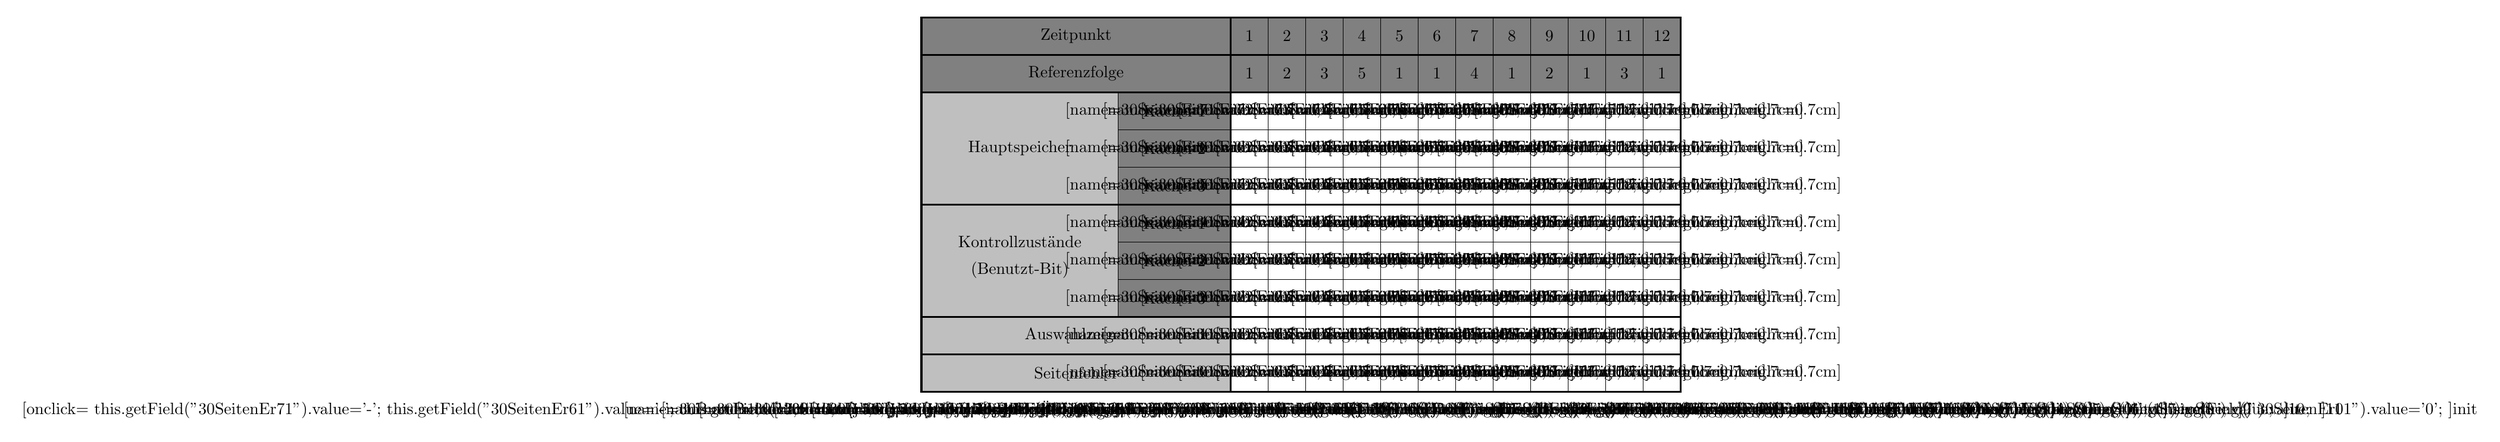
\begin{tikzpicture}
		\fill[fill=lightgray]
			(-1, 0.8) rectangle+(4.2, 4.8)
			(-1, -0.8) rectangle+(6.6, 1.6);
		\fill[fill=gray]
			(3.2, 0.8) rectangle+(2.4, 4.8)
			(-1, 5.6) rectangle+(16.2, 1.6);

		\draw (3.2, 4.8) -- (5.6, 4.8);
		\draw (3.2, 4) -- (5.6, 4);
		\draw (3.2, 2.4) -- (5.6, 2.4);
		\draw (3.2, 1.6) -- (5.6, 1.6);
		\draw (3.2, 0.8) -- (3.2, 5.6);
		\draw[step =.8cm] (5.6, -0.8) grid+(9.6, 8);
		\draw[very thick] (-1, -0.8) rectangle+(16.2, 8);
		\draw[very thick] (-1, 3.2) -- (15.2, 3.2);
		\draw[very thick] (-1, 0.8) -- (15.2, 0.8);
		\draw[very thick] (-1, 0) -- (15.2, 0);
		\draw[very thick] (-1, 6.4) -- (15.2, 6.4);
		\draw[very thick] (-1, 5.6) -- (15.2,5.6);
		\draw[very thick] (5.6, -0.8) -- (5.6, 7.2);

		\node at (2.3, 6.8) {Zeitpunkt};
		\node at (2.3, 6) {Referenzfolge};
		\node[text=black] at (1.1, 4.4) {Hauptspeicher};
		\node[text=black] at (1.1, 2.4) {Kontrollzustände};
		\node[text=black] at (1.1, 1.8) {(Benutzt-Bit)};
		\node at (4.4, 5.2) {Kachel 1};
		\node at (4.4, 4.4) {Kachel 2};
		\node at (4.4, 3.6) {Kachel 3};
		\node at (4.4, 2.8) {Kachel 1};
		\node at (4.4, 2) {Kachel 2};
		\node at (4.4, 1.2) {Kachel 3};
		\node[text=black] at (2.3, 0.4) {Auswahlzeiger};
		\node[text=black] at (2.3, -0.4) {Seitenfehler};
		\node at (2.3, -1.2) {Übertrage};
		%pageref
		\node at(6, 6.8) {1};
		\node at(6.8, 6.8) {2};
		\node at(7.6, 6.8) {3};
		\node at(8.4, 6.8) {4};
		\node at(9.2, 6.8) {5};
		\node at(10, 6.8) {6};
		\node at(10.8, 6.8) {7};
		\node at(11.6, 6.8) {8};
		\node at(12.4, 6.8) {9};
		\node at(13.2, 6.8) {10};
		\node at(14, 6.8) {11};
		\node at(14.8, 6.8) {12};
		%ref
		\node at(6, 6) {1};
		\node at(6.8, 6) {2};
		\node at(7.6, 6) {3};
		\node at(8.4, 6) {5};
		\node at(9.2, 6) {1};
		\node at(10, 6) {1};
		\node at(10.8, 6) {4};
		\node at(11.6, 6) {1};
		\node at(12.4, 6) {2};
		\node at(13.2, 6) {1};
		\node at(14, 6) {3};
		\node at(14.8, 6) {1};
		%HK1
		\foreach \j in {0,...,7}
		\foreach \i in {1,...,12}
		{
			\node at (5.105+0.8*\i, -0.4 + 0.8*\j) {\TextField[name=30SeitenEr\j\i,width=0.7cm,height=0.7cm]{\null}};
		}

		\node at (6.005, -1.2) {\PushButton[onclick={
				this.getField("30SeitenEr71").value='-';
				this.getField("30SeitenEr61").value='-';
				this.getField("30SeitenEr51").value='-';
				this.getField("30SeitenEr41").value='0';
				this.getField("30SeitenEr31").value='0';
				this.getField("30SeitenEr21").value='0';
				this.getField("30SeitenEr11").value='1';
				this.getField("30SeitenEr01").value='0';
			}]{init}};

		\foreach \i in{1,...,11}
		{
			\node at (6.005+0.8*\i, -1.2) {\PushButton[name=30Button\i,onclick={
			for(j=0; j<8; j++){
				this.getField(
					"30SeitenEr"+j.toString() + (\i+1).toString()
				).value=this.getField(
					"30SeitenEr"+j.toString() + (\i).toString()
				).value;
			}
			}]{\i}};
		}
	\end{tikzpicture}
\PushButton[onclick={
for(i=1; i< 13; i++) {
for(j=0; j<8; j++){
	this.getField("30SeitenEr" + j.toString() + i.toString()).value='';
}
}
}]{Clear}
\end{center}
\end{Form}
\end{samepage}
\end{beamerText}

\begin{normalText}

\begin{center}
	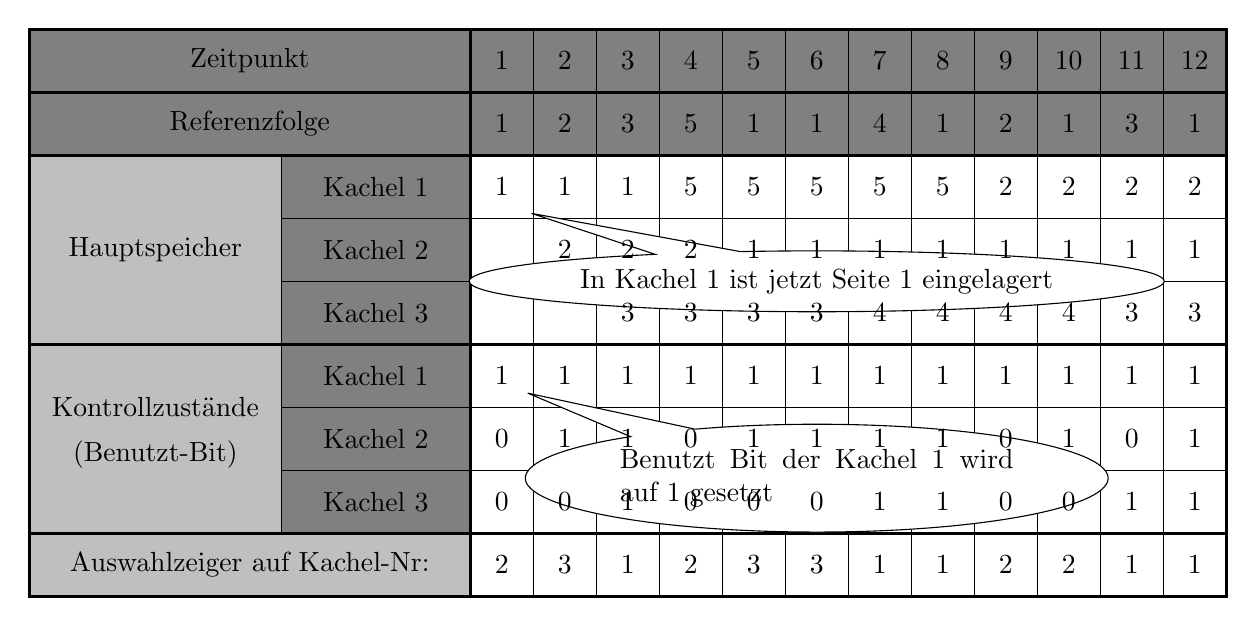
\begin{tikzpicture}
		\fill[fill=lightgray]
			(0, 0) rectangle+(3.2, 5.6)
			(3.2, 0) rectangle+(2.4, 0.8);
		\fill[fill=gray]
			(3.2, 0.8) rectangle+(2.4, 4.8)
			(0, 5.6) rectangle+(15.2, 1.6);

		\draw (3.2, 4.8) -- (5.6, 4.8);
		\draw (3.2, 4) -- (5.6, 4);
		\draw (3.2, 2.4) -- (5.6, 2.4);
		\draw (3.2, 1.6) -- (5.6, 1.6);
		\draw (3.2, 0.8) -- (3.2, 5.6);
		\draw[step =.8cm] (5.6, 0) grid+(9.6, 7.2);
		\draw[very thick] (0, 0) rectangle+(15.2, 7.2);
		\draw[very thick] (0, 3.2) -- (15.2, 3.2);
		\draw[very thick] (0, 0.8) -- (15.2, 0.8);
		\draw[very thick] (0, 6.4) -- (15.2, 6.4);
		\draw[very thick] (0, 5.6) -- (15.2,5.6);
		\draw[very thick] (5.6, 0) -- (5.6, 7.2);

		\node at (2.8, 6.8) {Zeitpunkt};
		\node at (2.8, 6) {Referenzfolge};
		\node at (1.6, 4.4) {Hauptspeicher};
		\node at (1.6, 2.4) {Kontrollzustände};
		\node at (1.6, 1.8) {(Benutzt-Bit)};
		\node at (4.4, 5.2) {Kachel 1};
		\node at (4.4, 4.4) {Kachel 2};
		\node at (4.4, 3.6) {Kachel 3};
		\node at (4.4, 2.8) {Kachel 1};
		\node at (4.4, 2) {Kachel 2};
		\node at (4.4, 1.2) {Kachel 3};
		\node at (2.8, 0.4) {Auswahlzeiger auf Kachel-Nr:};
		%pageref
		\node at(6, 6.8) {1};
		\node at(6.8, 6.8) {2};
		\node at(7.6, 6.8) {3};
		\node at(8.4, 6.8) {4};
		\node at(9.2, 6.8) {5};
		\node at(10, 6.8) {6};
		\node at(10.8, 6.8) {7};
		\node at(11.6, 6.8) {8};
		\node at(12.4, 6.8) {9};
		\node at(13.2, 6.8) {10};
		\node at(14, 6.8) {11};
		\node at(14.8, 6.8) {12};
		%ref
		\node at(6, 6) {1};
		\node at(6.8, 6) {2};
		\node at(7.6, 6) {3};
		\node at(8.4, 6) {5};
		\node at(9.2, 6) {1};
		\node at(10, 6) {1};
		\node at(10.8, 6) {4};
		\node at(11.6, 6) {1};
		\node at(12.4, 6) {2};
		\node at(13.2, 6) {1};
		\node at(14, 6) {3};
		\node at(14.8, 6) {1};
		%HK1
		\node at(6, 5.2) {1};
		\sol[{
			\node[shape=ellipse callout, callout relative pointer={(-2.1cm,0.5cm)},draw, fill=white] at (10,4) {In Kachel 1 ist jetzt Seite 1 eingelagert};
		}]{
			\node at(6.8, 5.2) {1};
			\node at(7.6, 5.2) {1};
			\node at(8.4, 5.2) {5};
			\node at(9.2, 5.2) {5};
			\node at(10, 5.2) {5};
			\node at(10.8, 5.2) {5};
			\node at(11.6, 5.2) {5};
			\node at(12.4, 5.2) {2};
			\node at(13.2, 5.2) {2};
			\node at(14, 5.2) {2};
			\node at(14.8, 5.2) {2};
			%HK2
			\node at(6.8, 4.4) {2};
			\node at(7.6, 4.4) {2};
			\node at(8.4, 4.4) {2};
			\node at(9.2, 4.4) {1};
			\node at(10, 4.4) {1};
			\node at(10.8, 4.4) {1};
			\node at(11.6, 4.4) {1};
			\node at(12.4, 4.4) {1};
			\node at(13.2, 4.4) {1};
			\node at(14, 4.4) {1};
			\node at(14.8, 4.4) {1};
			%HK3
			\node at(7.6, 3.6) {3};
			\node at(8.4, 3.6) {3};
			\node at(9.2, 3.6) {3};
			\node at(10, 3.6) {3};
			\node at(10.8, 3.6) {4};
			\node at(11.6, 3.6) {4};
			\node at(12.4, 3.6) {4};
			\node at(13.2, 3.6) {4};
			\node at(14, 3.6) {3};
			\node at(14.8, 3.6) {3};
			%ctrlK1
		}
		\node at(6, 2.8) {1};
		\sol[{
			\node[shape=ellipse callout, callout relative pointer={(-1.7cm,0.5cm)},draw, fill=white] at (10,1.5) {\parbox{5cm}{Benutzt Bit der Kachel 1 wird auf 1 gesetzt}};
		}]{
			\node at(6.8, 2.8) {1};
			\node at(7.6, 2.8) {1};
			\node at(8.4, 2.8) {1};
			\node at(9.2, 2.8) {1};
			\node at(10, 2.8) {1};
			\node at(10.8, 2.8) {1};
			\node at(11.6, 2.8) {1};
			\node at(12.4, 2.8) {1};
			\node at(13.2, 2.8) {1};
			\node at(14, 2.8) {1};
			\node at(14.8, 2.8) {1};
			%ctrlK2
			\node at(6, 2) {0};
			\node at(6.8, 2) {1};
			\node at(7.6, 2) {1};
			\node at(8.4, 2) {0};
			\node at(9.2, 2) {1};
			\node at(10, 2) {1};
			\node at(10.8, 2) {1};
			\node at(11.6, 2) {1};
			\node at(12.4, 2) {0};
			\node at(13.2, 2) {1};
			\node at(14, 2) {0};
			\node at(14.8, 2) {1};
			%ctrlK3
			\node at(6, 1.2) {0};
			\node at(6.8, 1.2) {0};
			\node at(7.6, 1.2) {1};
			\node at(8.4, 1.2) {0};
			\node at(9.2, 1.2) {0};
			\node at(10, 1.2) {0};
			\node at(10.8, 1.2) {1};
			\node at(11.6, 1.2) {1};
			\node at(12.4, 1.2) {0};
			\node at(13.2, 1.2) {0};
			\node at(14, 1.2) {1};
			\node at(14.8, 1.2) {1};
		}
		%pointer
		\node at(6, 0.4) {2};
		\sol{
			\node at(6.8, 0.4) {3};
			\node at(7.6, 0.4) {1};
			\node at(8.4, 0.4) {2};
			\node at(9.2, 0.4) {3};
			\node at(10, 0.4) {3};
			\node at(10.8, 0.4) {1};
			\node at(11.6, 0.4) {1};
			\node at(12.4, 0.4) {2};
			\node at(13.2, 0.4) {2};
			\node at(14, 0.4) {1};
			\node at(14.8, 0.4) {1};
		}
	\end{tikzpicture}
	\end{center}
\end{normalText}
\begin{solution}[Anzahl Seitenfehler: bisher 1 (Einlagern von Seite 1)]
	Anzahl Seitenfehler: bei Seitenreferenz 1, 2, 3, 5, 1, 4, 2, 3 also insgesamt 8

	Der Auswahlzeiger zeigt stets auf die Kachel, die für das Ersetzen als nächstes geprüft wird (sowohl wenn eine Seite eingefügt wurde, als auch wenn eine Seite schon im Puffer war und das Benutzt-Bit wieder auf 1 gesetzt wurde).

	Eignung von CLOCK: Ressourcenschonend, da lediglich ein Bit „Verwaltungsstruktur“ für jeden Puffer dazukommt, bzw. eine externe Bitmap mit der Anzahl der verwalteten Pufferblöcke geführt und durchsucht wird.
	CLOCK berücksichtigt jedoch nicht die Anzahl der Zugriffe.
	Jede Seite überlebt mindestens zwei „Zeigerumläufe“.
	Kann zu FIFO degenerieren, wenn alle Benutzt-Bits 1 sind (siehe Aufgabe).
	\subsection*{Ersetzungsverfahren und Lokalität}
\begin{minipage}{0.45\textwidth}
	Grundannahme bei Ersetzungsverfahren ist: Das Referenzverhalten der jüngsten Vergangenheit ist ähnlich dem der nächsten Zukunft $\rightarrow$ typischerweise hat man hohe Lokalität (d.h. in einem bestimmten Zeitintervall wird auf einem relativ kleinen Bereich Datenmenge gearbeitet). Hat man dagegen nur zufällige Zugriffe braucht man auch nicht Puffern -- bringt nichts, kostet nur ($\rightarrow$ Thrashing).
\end{minipage}
\begin{minipage}{0.5\textwidth}
	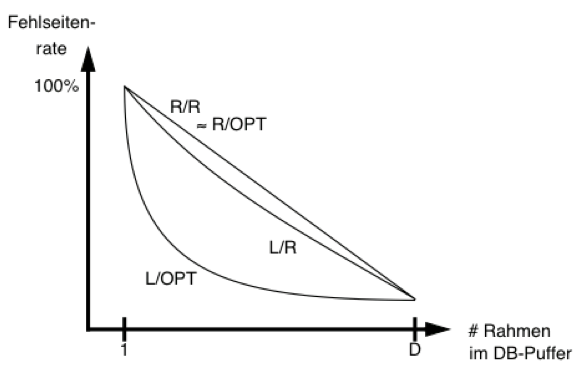
\includegraphics[width = 8cm]{Pictures/Ue07_Aufgabe2_Zusatz1.png}
\end{minipage}

\begin{tabular}{|l|l|l|l|l|}
	\hline
	 					& R/R 			& R/OPT 		& L/R 			& L/OPT 		\\
	\hline
	Referenzen 	& Random 	& Random 	& Lokalität 	& Lokalität 	\\
	\hline
	Ersetzung 	& Random 	& Opt 			& Random 	& Opt 			\\
	\hline
\end{tabular}

Belady-Optimal: Ersetze die Seite, die am längsten in die Zukunft nicht referenziert wird.
\end{solution}

\begin{beamerText}
\pagebreak
\subsection*{Ersetzungsverfahren und Lokalität}
\begin{minipage}{0.45\textwidth}
	Grundannahme bei Ersetzungsverfahren ist: Das Referenzverhalten der jüngsten Vergangenheit ist ähnlich dem der nächsten Zukunft $\rightarrow$ typischerweise hat man hohe Lokalität (d.h. in einem bestimmten Zeitintervall wird auf einem relativ kleinen Bereich Datenmenge gearbeitet). Hat man dagegen nur zufällige Zugriffe braucht man auch nicht Puffern -- bringt nichts, kostet nur ($\rightarrow$ Thrashing).
\end{minipage}
\begin{minipage}{0.5\textwidth}
	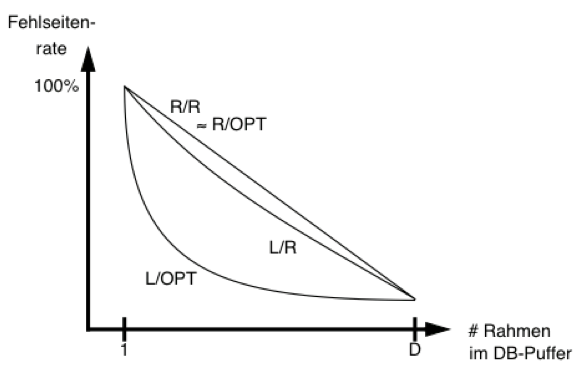
\includegraphics[width = 8cm]{Pictures/Ue07_Aufgabe2_Zusatz1.png}
\end{minipage}

\begin{tabular}{|l|l|l|l|l|}
	\hline
	 					& R/R 			& R/OPT 		& L/R 			& L/OPT 		\\
	\hline
	Referenzen 	& Random 	& Random 	& Lokalität 	& Lokalität 	\\
	\hline
	Ersetzung 	& Random 	& Opt 			& Random 	& Opt 			\\
	\hline
\end{tabular}

Belady-Optimal: Ersetze die Seite, die am längsten in die Zukunft nicht referenziert wird.
\pagebreak
\end{beamerText}

\item Gegeben ist die folgende Seitenreferenzfolge für die Zeitpunkte \(t=1\) bis \(t=13\):
\(1, 2, 1, 3, 1, 2, 1, 2, 3, 4, 5, 6, 7\)

Bestimmen Sie die Working Set Size und die aktuelle Lokalität für eine Fenstergröße von \(w = 8\) für die Zeitpunkte \(t=8\) und \(t=13\).
Bestimmen Sie weiterhin die durchschnittliche Lokalität für diese Fenstergröße und die gegebene Referenzfolge.

\begin{solution}
Die Anzahl an unterschiedlichen referenzierten Seiten bei $w$ Zugriffen nennen wir Working Set Size.
Betrachten wir  die ersten 8 (\(t=8: (1,2,1,3,1,2,1,2)\)) und die letzten 8 Zugriffe (\(t=13: (2,1,2,3,4,5,6,7)\)), dann sehen wir, dass im ersten Fall 3 unterschiedliche Werte auftreten und im anderen Fall 7 $\rightarrow$ die Working Set Size $|W|$ beträgt im ersten Fall also $3$ und im zweiten Fall $7$.

Die aktuelle Lokalität ist dann gegeben durch	\[AL(t, w) = \frac{|W(t, w)|}{w}\] d.\,h. $\frac{3}{8}$
für \(t=8\), und $\frac{7}{8}$ für \(t=13\).

Die durchschnittliche Lokalität ist: \[L(w) = \frac{\sum_{t = w}^n AL(t, w)}{n-(w-1)}\]
Für die gegebene Referenzfolge ergibt sich eine durchschnittliche Lokalität von:
\begin{equation*}
	 L(8) = \frac{\sum_{t = 8}^{13} AL(t, 8)}{6} = \frac{1}{6} \cdot (\frac{3}{8}+\frac{3}{8}+\frac{4}{8}+\frac{5}{8}+\frac{6}{8}+\frac{7}{8}) = \frac{7}{12}
\end{equation*}

\end{solution}

    \item Bestimmen Sie für die Seitenreferenzfolge $1, 2, 3, 5, 1, 1, 4, 1, 2, 1, 3, 1$ die LRU-Stack\-tie\-fen\-ver\-tei\-lung.

\begin{solution}
Der LRU-Stack enthält alle bereits referenzierten Seiten in der Reihenfolge ihres Zugriffsalters.
Wie bestimmt man die Stacktiefen-Verteilung? Pro Stackposition gibt es einen Zähler; Referenz einer Seite führt zu Zählererhöhung an der jew. Stackposition ($\rightarrow$ Zählerwerte entsprechen Wiederbenutzungshäufigkeit)


    \begin{minipage}{0.28\textwidth}
        \center
        Zugriff auf 1, 2, 3, 5:

        \begin{tabular}{ | c | l}
        	\cline{1-1}
        	5      & 0      \\ \cline{1-1}
        	3      & 0      \\ \cline{1-1}
        	2      & 0      \\ \cline{1-1}
        	1      & 0      \\ \cline{1-1}
        	       & 0      \\ \cline{1-1}
        	\vdots & \vdots \\ \cline{1-1}
        \end{tabular}
    \end{minipage}
    \begin{minipage}{0.22\textwidth}
        \center
        Zugriff auf 1:

        \begin{tabular}{ | c | l}
        	\cline{1-1}
        	1      & 0      \\ \cline{1-1}
        	5      & 0      \\ \cline{1-1}
        	3      & 0      \\ \cline{1-1}
        	2      & 1      \\ \cline{1-1}
        	       & 0      \\ \cline{1-1}
        	\vdots & \vdots \\ \cline{1-1}
        \end{tabular}
    \end{minipage}
    \begin{minipage}{0.22\textwidth}
        \center
        Zugriff auf 1:

        \begin{tabular}{ | c | l}
        	\cline{1-1}
        	1      & 1      \\ \cline{1-1}
        	5      & 0      \\ \cline{1-1}
        	3      & 0      \\ \cline{1-1}
        	2      & 1      \\ \cline{1-1}
        	       & 0      \\ \cline{1-1}
        	\vdots & \vdots \\ \cline{1-1}
        \end{tabular}
    \end{minipage}
    \begin{minipage}{0.22\textwidth}
        \center
        Zugriff auf 4:

        \begin{tabular}{ | c | l}
        	\cline{1-1}
        	4      & 1      \\ \cline{1-1}
        	1      & 0      \\ \cline{1-1}
        	5      & 0      \\ \cline{1-1}
        	3      & 1      \\ \cline{1-1}
        	2      & 0      \\ \cline{1-1}
        	       & 0      \\ \cline{1-1}
        	\vdots & \vdots \\ \cline{1-1}
        \end{tabular}
    \end{minipage}

    \begin{minipage}{0.28\textwidth}
        \center
        Zugriff auf 1:

        \begin{tabular}{ | c | l}
        	\cline{1-1}
        	1      & 1      \\ \cline{1-1}
        	4      & 1      \\ \cline{1-1}
        	5      & 0      \\ \cline{1-1}
        	3      & 1      \\ \cline{1-1}
        	2      & 0      \\ \cline{1-1}
        	       & 0      \\ \cline{1-1}
        	\vdots & \vdots \\ \cline{1-1}
        \end{tabular}
    \end{minipage}
    \begin{minipage}{0.22\textwidth}
        \center
        Zugriff auf 2:

        \begin{tabular}{ | c | l}
        	\cline{1-1}
        	2      & 1      \\ \cline{1-1}
        	1      & 1      \\ \cline{1-1}
        	4      & 0      \\ \cline{1-1}
        	5      & 1      \\ \cline{1-1}
        	3      & 1      \\ \cline{1-1}
        	       & 0      \\ \cline{1-1}
        	\vdots & \vdots \\ \cline{1-1}
        \end{tabular}
    \end{minipage}
    \begin{minipage}{0.22\textwidth}
        \center
        Zugriff auf 1:

        \begin{tabular}{ | c | l}
        	\cline{1-1}
        	1      & 1      \\ \cline{1-1}
        	2      & 2      \\ \cline{1-1}
        	4      & 0      \\ \cline{1-1}
        	5      & 1      \\ \cline{1-1}
        	3      & 1      \\ \cline{1-1}
        	       & 0      \\ \cline{1-1}
        	\vdots & \vdots \\ \cline{1-1}
        \end{tabular}
    \end{minipage}
    \begin{minipage}{0.22\textwidth}
        \center
        Zugriff auf 3:

        \begin{tabular}{ | c | l}
        	\cline{1-1}
        	3      & 1      \\ \cline{1-1}
        	1      & 2      \\ \cline{1-1}
        	2      & 0      \\ \cline{1-1}
        	4      & 1      \\ \cline{1-1}
        	5      & 2      \\ \cline{1-1}
        	       & 0      \\ \cline{1-1}
        	\vdots & \vdots \\ \cline{1-1}
        \end{tabular}
    \end{minipage}

        \begin{minipage}{0.28\textwidth}
            \center
            Zugriff auf 1:

            \begin{tabular}{ | c | l}
            	\cline{1-1}
            	1      & 1      \\ \cline{1-1}
            	3      & 3      \\ \cline{1-1}
            	2      & 0      \\ \cline{1-1}
            	4      & 1      \\ \cline{1-1}
            	5      & 2      \\ \cline{1-1}
            	       & 0      \\ \cline{1-1}
            	\vdots & \vdots \\ \cline{1-1}
            \end{tabular}
        \end{minipage}
        \begin{minipage}{0.65\textwidth}
            Endergebnis (von oberster zu niedrigster Stackposition):

						1, 3, 0, 1, 2
        \end{minipage}

\end{solution}

\item Welche Informationen liefert die LRU-Stacktiefenverteilung?

\begin{solution}
Für das Ersetzungsverfahren LRU können aus der Stacktiefenverteilung für eine bestimmte Puffergröße direkt die Treffer- und Fehlseitenrate bestimmt werden.
Für eine beispielhafte Puffergröße von 3 im oberen Beispiel hätte LRU 1+3+0 = 4 Treffer und 1+2 = 3 Fehler beim Zugriff.

Charakteristisch ist die starke, oft monotone Abnahme der Wiederbenutzungswahrscheinlichkeit mit der Stacktiefe.
Seitenreferenzen folgen oft der 80/20-Regel (20\,\% der Seiten vereinen 80\,\% der Zugriffe auf sich, die restlichen 80\,\% der Seiten nur 20\,\% der Zugriffe) oder besitzen noch ausgeprägtere Lokalität.

\begin{center}
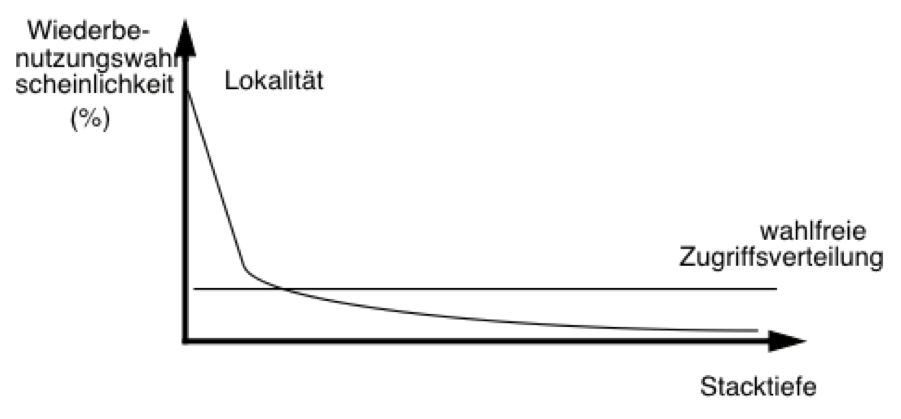
\includegraphics[width = 10cm]{Pictures/Ue07_Aufgabe2_Zusatz2.png}
\end{center}

Ausnahmen in der Monotonie können z.B. durch das Schreiben ins Log oder Warten auf Sperren auftreten.
\end{solution}

%\item Was sind die Grundideen der in der Vorlesung vorgestellten Ersetzungsstrategien? \\Was sind die Vor- und Nachteile dieser einzelnen Strategien?
%
%\begin{note}
%	Evtl Vorstellung mit Skizze: \\
%	FIFO: Stack mit \glqq Ersetzungzeiger\grqq\\
%	LFU: Nach Zugriffen sortierte Liste (Mit Counter)\\
%	LRU: Nach Letztem Zugriffsalter Sortierte Liste (Jeder benutze Block kommt nach ganz oben)\\
%	CLOCK: Uhr anzeichnen mit Benutzt-Bit
%\end{note}
%
%\begin{solution}
%\begin{tabular}{|c|p{6cm}|p{6cm}|}
%	\hline
%	& Welche Blöcke werden verdrängt? &Vor- und Nachteile \\
%	\hline
%	FIFO & Der Block, der am Längsten im Puffer liegt wird verdrängt. & Häufig genutzte Blöcke verschwinden schnell aus dem Puffer. \\
%	\hline
%	LFU & Der Block, der am wenigsten genutzt wurde wird verdrängt. & Einmal häufig genutzte Blöcke verschwinden nie aus dem Puffer. \\
%	\hline
%	LRU & Der Block, der am Längsten nicht genutzt wurde wird verdrängt. & Stapelverwaltung sehr aufwändig. \\
%	\hline
%	CLOCK &   Der Block, auf welchen der Zeiger das nächste mal zeigt und welcher seit dem letzten Zeigerdurchlauf nicht genutzt wurde. & Nicht so gut wie LRU aber deutlich effizienter. \\
%	\hline
%\end{tabular}
%\end{solution}


\end{enumerate}


\beamertxt{\pagebreak}
\begin{selbstTest}
\section{Seitenersetzung Teil 2}
Für einen Puffer wie in Aufgabe \ref{Seiten} stehen vier Seiten im Hauptspeicher zur Verfügung.
\begin{enumerate}[a)]
	\item Stellen Sie nun den Zustand des Puffers zur gegebenen Seitenreferenzenfolge für alle vier in der Vorlesung vorgestellten Seitenersetzungsstrategien dar.

	Reihenfolge der Seitenreferenzen: 1, 4, 1, 4, 2, 1, 3, 5, 6, 2, 3, 7, 3, 10, 9, 5, 10, 4, 8, 8

\begin{normalText}
	Beispiele zur Notation:


	\begin{minipage}{.49\textwidth}
		FIFO:

		\vspace{.25cm}

		\begin{tabular}{|p{4.3cm}||c|c|c|}
			\hline
			\rowcolor{gray} Zeitpunkt & 1 & 2 & 3 \\
			\hline
			\rowcolor{gray} Referenzfolge & 1 & 4 & 1 \\
			\hline \hline
			Kachel 1 & 1 & 1 & 1 \\
			\hline
			Kachel 2 & - & 4 & 4 \\
			\hline
			Kachel 3 & - & - & - \\
			\hline
			Kachel 4 & - & - & - \\
			\hline \hline
			\rowcolor{lightgray} \raggedright Auswahlzeiger auf Kachel-Nr: & 2 & 3 & 3 \\
			\hline\hline
			\rowcolor{gray} Seitenfehler & 1 & 2 & 2 \\
			\hline
		\end{tabular}
	\end{minipage}
	\begin{minipage}{.45\textwidth}
		LFU:

		\vspace{.25cm}

		\begin{tabular}{|p{4.3cm}||c|c|c|}
			\hline
			\rowcolor{gray} Zeitpunkt & 1 & 2 & 3 \\
			\hline
			\rowcolor{gray} Referenzfolge & 1 & 4 & 1 \\
			\hline \hline
			Kachel 1 & 1 & 1 & 1 \\
			\hline
			Kachel 2 & - & 4 & 4 \\
			\hline
			Kachel 3 & - & - & - \\
			\hline
			Kachel 4 & - & - & - \\
			\hline \hline
			\rowcolor{lightgray} Zugriffszähler Kachel 1 & 1 & 1 & 2 \\
			\hline
			\rowcolor{lightgray} Zugriffszähler Kachel 2 & - & 1 & 1 \\
			\hline
			\rowcolor{lightgray} Zugriffszähler Kachel 3 & - & - & - \\
			\hline
			\rowcolor{lightgray} Zugriffszähler Kachel 4 & - & - & - \\
			\hline \hline
			\rowcolor{gray} Seitenfehler & 1 & 2 & 2 \\
			\hline
		\end{tabular}
	\end{minipage}

	\begin{minipage}{.49\textwidth}
		LRU:

		\vspace{.25cm}

		\begin{tabular}{|p{4.3cm}||c|c|c|}
			\hline
			\rowcolor{gray} Zeitpunkt & 1 & 2 & 3 \\
			\hline
			\rowcolor{gray} Referenzfolge & 1 & 4 & 1 \\
			\hline \hline
			Kachel 1 & 1 & 1 & 1 \\
			\hline
			Kachel 2 & - & 4 & 4 \\
			\hline
			Kachel 3 & - & - & - \\
			\hline
			Kachel 4 & - & - & - \\
			\hline \hline
			\rowcolor{lightgray} Letzter Zugriff Kachel 1 & 1 & 1 & 3 \\
			\hline
			\rowcolor{lightgray} Letzter Zugriff Kachel 2 & - & 2 & 2 \\
			\hline
			\rowcolor{lightgray} Letzter Zugriff Kachel 3 & - & - & - \\
			\hline
			\rowcolor{lightgray} Letzter Zugriff Kachel 4 & - & - & - \\
			\hline \hline
			\rowcolor{gray} Seitenfehler & 1 & 2 & 2 \\
			\hline
		\end{tabular}
	\end{minipage}
	\begin{minipage}{.45\textwidth}
		CLOCK:

		\vspace{.25cm}

		\begin{tabular}{|p{4.3cm}||c|c|c|}
			\hline
			\rowcolor{gray} Zeitpunkt & 1 & 2 & 3 \\
			\hline
			\rowcolor{gray} Referenzfolge & 1 & 4 & 1 \\
			\hline \hline
			Kachel 1 & 1 & 1 & 1 \\
			\hline
			Kachel 2 & - & 4 & 4 \\
			\hline
			Kachel 3 & - & - & - \\
			\hline
			Kachel 4 & - & - & - \\
			\hline \hline
			\rowcolor{lightgray}Kontrollzustand Kachel 1 & 1 & 1 & 1 \\
			\hline
			\rowcolor{lightgray}Kontrollzustand Kachel 2 & 0 & 1 & 1 \\
			\hline
			\rowcolor{lightgray}Kontrollzustand Kachel 3 & 0 & 0 & 0 \\
			\hline
			\rowcolor{lightgray}Kontrollzustand Kachel 4 & 0 & 0 & 0 \\
			\hline
			\rowcolor{lightgray} \raggedright Auswahlzeiger auf Kachel-Nr: & 2 & 3 & 3 \\
			\hline\hline
			\rowcolor{gray} Seitenfehler & 1 & 2 & 2 \\
			\hline
		\end{tabular}
	\end{minipage}
\end{normalText}

\cprotEnv
\begin{solution}
Sie können ihre Lösung gerne mithilfe des Web-Tools \url{http://faui6g.informatik.uni-erlangen.de/#/paging} selbstständig überprüfen.
\end{solution}

\cprotEnv
\begin{note}
FIFO:\nopagebreak

\begin{tabular}{|c||c|c|c|c|c|c|c|c|c|c|c|c|c|c|c|c|c|c|c|c|}
	\hline
	\rowcolor{lightgray} Refnr & 1 & 2 & 3 & 4 & 5 & 6 & 7 & 8 & 9 & 10 & 11 & 12 & 13 & 14 & 15 & 16 & 17 & 18 & 19 & 20 \\
	\hline
	\rowcolor{lightgray} Ref & 1 & 4 & 1 & 4 & 2 & 1 & 3 & 5 & 6 & 2 & 3 & 7 & 3 & 10 & 9 & 5 & 10 & 4 & 8 & 8 \\
	\hline \hline
	K 1 & \color{blue} 1 & 1 & \color{blue} 1 & 1 & 1 & \color{blue} 1 & 1 & \color{blue} 5 & 5 & 5 & 5 & 5 & 5 & 5 & \color{blue} 9 & 9 & 9 & 9 & 9 & 9 \\
	\hline
	K 2 & - & \color{blue} 4 & 4 & \color{blue} 4 & 4 & 4 & 4 & 4 & \color{blue} 6 & 6 & 6 & 6 & 6 & 6 & 6 & \color{blue} 5 & 5 & 5 & 5 & 5 \\
	\hline
	K 3 & - & - & - & - & \color{blue} 2 & 2 & 2 & 2 & 2 & \color{blue} 2 & 2 & \color{blue} 7 & 7 & 7 & 7 & 7 & 7 & \color{blue} 4 & 4 & 4 \\
	\hline
	K 4 & - & - & - & - & - & - & \color{blue} 3 & 3 & 3 & 3 & \color{blue} 3 & 3 & \color{blue} 3 & \color{blue} 10 & 10 & 10 & \color{blue} 10 & 10 & \color{blue} 8 & \color{blue} 8 \\
	\hline \hline
	\rowcolor{lightgray} Next & 2 & 3 & 3 & 3 & 4 & 4 & 1 & 2 & 3 & 3 & 3 & 4 & 4 & 1 & 2 & 3 & 3 & 4 & 1 & 1 \\
	\hline
	Fehler & 1 & 2 & 2 & 2 & 3 & 3 & 4 & 5 & 6 & 6 & 6 & 7 & 7 & 8 & 9 & 10 & 10 & 11 & 12 & 12 \\
	\hline
\end{tabular}

LFU:\nopagebreak

\begin{tabular}{|c||c|c|c|c|c|c|c|c|c|c|c|c|c|c|c|c|c|c|c|c|}
	\hline
	\rowcolor{lightgray} Refnr & 1 & 2 & 3 & 4 & 5 & 6 & 7 & 8 & 9 & 10 & 11 & 12 & 13 & 14 & 15 & 16 & 17 & 18 & 19 & 20 \\
	\hline
	\rowcolor{lightgray} Ref & 1 & 4 & 1 & 4 & 2 & 1 & 3 & 5 & 6 & 2 & 3 & 7 & 3 & 10 & 9 & 5 & 10 & 4 & 8 & 8 \\
	\hline \hline
	K 1 & \color{blue} 1 & 1 & \color{blue} 1 & 1 & 1 & \color{blue} 1 & 1 & 1 & 1 & 1 & 1 & 1 & 1 & 1 & 1 & 1 & 1 & 1 & 1 & 1 \\
	\hline
	K 2 & - & \color{blue} 4 & 4 & \color{blue} 4 & 4 & 4 & 4 & 4 & 4 & 4 & 4 & 4 & 4 & 4 & 4 & 4 & 4 & \color{blue} 4 & 4 & 4 \\
	\hline
	K 3 & - & - & - & - & \color{blue} 2 & 2 & 2 & \color{blue} 5 & 5 & \color{blue} 2 & 2 & \color{blue} 7 & 7 & \color{blue} 10 & \color{blue} 9 & \color{blue} 5 & \color{blue} 10 & 10 & \color{blue} 8 & \color{blue} 8 \\
	\hline
	K 4 & - & - & - & - & - & - & \color{blue} 3 & 3 & \color{blue} 6 & 6 & \color{blue} 3 & 3 & \color{blue} 3 & 3 & 3 & 3 & 3 & 3 & 3 & 3 \\
	\hline \hline
	\rowcolor{lightgray} Z 1 & \color{blue} 1 & 1 & \color{blue} 2 & 2 & 2 & \color{blue} 3 & 3 & 3 & 3 & 3 & 3 & 3 & 3 & 3 & 3 & 3 & 3 & 3 & 3 & 3 \\
	\hline
	\rowcolor{lightgray} Z 2 & - & \color{blue} 1 & 1 & \color{blue} 2 & 2 & 2 & 2 & 2 & 2 & 2 & 2 & 2 & 2 & 2 & 2 & 2 & 2 & \color{blue} 3 & 3 & 3 \\
	\hline
	\rowcolor{lightgray} Z 3 & - & - & - & - & \color{blue} 1 & 1 & 1 & \color{blue} 1 & 1 & \color{blue} 1 & 1 & \color{blue} 1 & 1 & \color{blue} 1 & \color{blue} 1 & \color{blue} 1 & \color{blue} 1 & 1 & \color{blue} 1 & \color{blue} 2 \\
	\hline
	\rowcolor{lightgray} Z 4 & - & - & - & - &  &  & \color{blue} 1 & 1 & \color{blue} 1 & 1 & \color{blue} 1 & 1 & \color{blue} 2 & 2 & 2 & 2 & 2 & 2 & 2 & 2 \\
	\hline \hline
	Fehler & 1 & 2 & 2 & 2 & 3 & 3 & 4 & 5 & 6 & 7 & 8 & 9 & 9 & 10 & 11 & 12 & 13 & 13 & 14 & 14 \\
	\hline
\end{tabular}

LRU:\nopagebreak

\begin{tabular}{|c||c|c|c|c|c|c|c|c|c|c|c|c|c|c|c|c|c|c|c|c|}
	\hline
	\rowcolor{lightgray} Refnr & 1 & 2 & 3 & 4 & 5 & 6 & 7 & 8 & 9 & 10 & 11 & 12 & 13 & 14 & 15 & 16 & 17 & 18 & 19 & 20 \\
	\hline
	\rowcolor{lightgray} Ref. & 1 & 4 & 1 & 4 & 2 & 1 & 3 & 5 & 6 & 2 & 3 & 7 & 3 & 10 & 9 & 5 & 10 & 4 & 8 & 8 \\
	\hline \hline
	K 1 & \color{blue} 1 & 1 & \color{blue} 1 & 1 & 1 & \color{blue} 1 & 1 & 1 & 1 & \color{blue} 2 & 2 & 2 & 2 & 2 & \color{blue} 9 & 9 & 9 & 9 & \color{blue} 8 & \color{blue} 8 \\
	\hline
	K 2 & - & \color{blue} 4 & 4 & \color{blue} 4 & 4 & 4 & 4 & \color{blue} 5 & 5 & 5 & 5 & \color{blue} 7 & 7 & 7 & 7 & \color{blue} 5 & 5 & 5 & 5 & 5 \\
	\hline
	K 3 & - & - & - & - & \color{blue} 2 & 2 & 2 & 2 & \color{blue} 6 & 6 & 6 & 6 & 6 & \color{blue} 10 & 10 & 10 & \color{blue} 10 & 10 & 10 & 10 \\
	\hline
	K 4 & - & - & - & - & - & - & \color{blue} 3 & 3 & 3 & 3 & \color{blue} 3 & 3 & \color{blue} 3 & 3 & 3 & 3 & 3 & \color{blue} 4 & 4 & 4 \\
	\hline \hline
	\rowcolor{lightgray} Z 1 & \color{blue} 1 & 1 & \color{blue} 3 & 3 & 3 & \color{blue} 6 & 6 & 6 & 6 & \color{blue} 10 & 10 & 10 & 10 & 10 & \color{blue} 15 & 15 & 15 & 15 & \color{blue} 19 & \color{blue} 20 \\
	\hline
	\rowcolor{lightgray} Z 2 & - & \color{blue} 2 & 2 & \color{blue} 4 & 4 & 4 & 4 & \color{blue} 8 & 8 & 8 & 8 & \color{blue} 12 & 12 & 12 & 12 & \color{blue} 16 & 16 & 16 & 16 & 16 \\
	\hline
	\rowcolor{lightgray} Z 3 & - & - & - & - & \color{blue} 5 & 5 & 5 & 5 & \color{blue} 9 & 9 & 9 & 9 & 9 & \color{blue} 14 & 14 & 14 & \color{blue} 17 & 17 & 17 & 17 \\
	\hline
	\rowcolor{lightgray} Z 4 & - & - & - & - & - & - & \color{blue} 7 & 7 & 7 & 7 & \color{blue} 11 & 11 & \color{blue} 13 & 13 & 13 & 13 & 13 & \color{blue} 18 & 18 & 18 \\
	\hline \hline
	Fehler & 1 & 2 & 2 & 2 & 3 & 3 & 4 & 5 & 6 & 7 & 7 & 8 & 8 & 9 & 10 & 11 & 11 & 12 & 13 & 13 \\
	\hline
\end{tabular}

Clock:\nopagebreak

\begin{tabular}{|c||c|c|c|c|c|c|c|c|c|c|c|c|c|c|c|c|c|c|c|c|}
	\hline
	\rowcolor{lightgray} Refnr & 1 & 2 & 3 & 4 & 5 & 6 & 7 & 8 & 9 & 10 & 11 & 12 & 13 & 14 & 15 & 16 & 17 & 18 & 19 & 20 \\
	\hline
	\rowcolor{lightgray} Ref & 1 & 4 & 1 & 4 & 2 & 1 & 3 & 5 & 6 & 2 & 3 & 7 & 3 & 10 & 9 & 5 & 10 & 4 & 8 & 8 \\
	\hline \hline
	K 1 & \color{blue} 1 & 1 & \color{blue} 1 & 1 & 1 & \color{blue} 1 & 1 & \color{blue} 5 & 5 & 5 & 5 & 5 & 5 & \color{blue} 10 & 10 & 10 & \color{blue} 10 & 10  & \color{blue} 8 &  \color{blue} 8 \\
	\hline
	K 2 & - & \color{blue} 4 & 4 & \color{blue} 4 & 4 & 4 & 4 & 4 & \color{blue} 6 & 6 & 6 & 6 & 6 & 6 & \color{blue} 9 & 9 & 9 & 9 & 9 & 9 \\
	\hline
	K 3 & - & - & - & - & \color{blue} 2 & 2 & 2 & 2 & 2 & \color{blue} 2 & 2 & \color{blue} 7 & 7 & 7 & 7 & 7 & 7 & \color{blue} 4 & 4 & 4 \\
	\hline
	K 4 & - & - & - & - & - & - & \color{blue} 3 & 3 & 3 & 3 & \color{blue} 3 & 3 & \color{blue} 3 & 3 & 3 & \color{blue} 5 & 5 & 5 & 5 & 5 \\
	\hline \hline
	\rowcolor{lightgray} Z 1 & \color{blue} 1 & 1 & \color{blue} 1 & 1 & 1 & \color{blue} 1 & 1 & \color{blue} 1 & 1 & 1 & 1 & 0  & 0 & \color{blue} 1 & 1 & 1 & \color{blue} 1 & 0 & \color{blue} 1 & \color{blue} 1 \\
	\hline
	\rowcolor{lightgray} Z 2 & 0 & \color{blue} 1 & 1 & \color{blue} 1 & 1 & 1 & 1 & 0 & \color{blue} 1 & 1 & 1 & 0 & 0 & 0 & \color{blue} 1 & 1 & 1 & 0 & 0 & 0 \\
	\hline
	\rowcolor{lightgray} Z 3 & 0 & 0 & 0 & 0 & \color{blue} 1 & 1 & 1 & 0 & 0 & \color{blue} 1 & 1 & \color{blue} 1 & 1 & 1 & 1 & 0 & 0 & \color{blue} 1 & 1 & 1 \\
	\hline
	\rowcolor{lightgray} Z 4 & 0 & 0 & 0 & 0 & 0 & 0 & \color{blue} 1 & 0 & 0 & 0 & \color{blue} 1 & 0 & \color{blue} 1 & 0 & 0 & \color{blue} 1 & 1 & 1 & 0 & 0 \\
	\hline \hline
	Zeig & 2 & 3 & 3 & 3 & 4 & 4 & 1 & 2 & 3 & 3 & 3 & 4 & 4 & 2 & 3 & 1 & 1 & 4 & 2 & 2 \\
	\hline
	Fehler & 1 & 2 & 2 & 2 & 3 & 3 & 4 & 5 & 6 & 6 & 6 & 7 & 7 & 8 & 9 & 10 & 10 & 11 & 12 & 12 \\
	\hline
\end{tabular}
\end{note}
	\item Welche \deepen Strategie eignet sich Ihrer Meinung nach am besten und wieso?

	\begin{note}
		CLOCK hat, genauso wie FIFO in diesem Fall nur 12 Seitenfehler. Der Verwaltungsaufwand ist bei diesen beiden annähernd identisch.
	\end{note}
\end{enumerate}

\end{selbstTest}

\beamertxt{\pagebreak}
\section{Pufferverwaltung}
Die Pufferverwaltung bestimmt, welche Seiten im Puffer gehalten werden. Um die Seiten im Puffer wiederfinden zu können, muss sie auch verwalten, welche Seiten gerade im Puffer liegen und wo. Benötigt wird z.\,B. eine Funktion wie die folgende:

\texttt{/* liefert entweder die Adresse der Seite im Puffer \beamertxt{\linebreak}
oder null, wenn die \normaltxt{\linebreak}
Seite nicht im Puffer liegt */\\
	void* findPage(int pageNo); }

Mittels welcher Hilfsstrukturen könnte man so eine Funktion implementieren? Denken Sie an Ihnen bekannte Datenstrukturen sowie die Verfahren zur Satzadressierung, die wir in dieser Veranstaltung kennengelernt haben. Welche dieser Strukturen sind gut geeignet? Berücksichtigen Sie folgende Randbedingungen:
\begin{itemize}
	\item Die Suche im Puffer kommt relativ häufig vor, muss also schnell gehen.
	\item Das Einfügen oder Löschen einer Seite im Puffer kommt etwa 1--2 Größenordnungen seltener vor als die Suche, also immer noch häufig. In diesem Fall muss außerdem die neue Seite vom Hintergrundspeicher geladen werden.
\end{itemize}

\begin{solution}
\underline{Hinweis:} Bei der Laufzeit des Löschens nehmen wir an, dass wir den Eintrag in der jeweiligen Struktur bereits gefunden haben.
\begin{itemize}
	\item Einfachste Idee: man schreibt die Nummer der Seite, die in einer Kachel liegt, direkt mit in die Kachel. Zur Suche durchläuft man alle Kacheln sequentiell. Das hat zwei gravierende Nachteile:
	\begin{itemize}
		\item Die Kacheln müssen jetzt um ein geringes größer sein als eine Seite. Das führt zu Caching-Problemen (die Kachelgrenzen fallen z.B. nicht mehr auf Betriebssystem-Seitengrenzen).

		\item Außerdem kann uns die Speicherverwaltung des BS ja Seiten in den Hintergrundspeicher auslagern. Wenn wir nun in einer Kachel nachschauen, welche Seite drin ist, muss das BS sie evtl. erst wieder einlagern. Das ist viel zu teuer.
	\end{itemize}
	Aufwände: Suche: O(n), Ändern O(1)

	\item Verbesserung: da wir die Seitennummern nicht in die Kacheln schreiben können, ziehen wir sie in eine eigene Verwaltungsstruktur heraus. Das kann z.\,B. eine Liste sein. Da i.\,A. die Puffergröße fest ist, kann man ein einfaches Array verwenden, das genauso viele Einträge hat wie der Puffer Kacheln. Hier gibt es nun zwei Varianten: a) unsortiert oder b) sortiert (nach Seitennummer).

	Aufwände: a) Suche: O(n), Ändern O(1); b) Suche: O($log_2(n)$) (binäre Suche), Ändern O(n) (Es muss im Mittel die Hälfte der Einträge nach unten verschoben werden.), meist besser, da Suche häufiger als Änderung.

	\item Verkettete Liste: Einfügen/Löschen geht in O(1) (da man nicht mehr umkopieren muss, sondern nur zwei Zeiger umbiegen), Suche in O(n) (Liste kann zwar sortiert sein, aber man kann nicht mehr binär suchen. Bei Misserfolg im Mittel n/2 wenn sortiert, sonst n.

	\item In Analogie zu DBTT kann man die Liste umkehren: Jede denkbare Seite bekommt einen Eintrag und man kann direkt nachschauen, wo die Seite liegt.

	Aufwände: Suche O(1), Ändern O(1).

	Gravierender Nachteil: Die Größe der Tabelle. Sie wird in der Größenordnung von 1/1000 der gesamten Datenbankgröße liegen. Für ein Terabyte Daten muss man also mit der Größenordnung von 1\,GB für die Tabelle rechnen (und die muss immer im Speicher liegen). Das ist nicht praktikabel.

	\item Eine Analogie zu TID erscheint nicht sinnvoll.

	\item Hashing: Für diesen Zweck das beste Verfahren, das auch häufig verwendet wird. Üblicherweise in der Variante mit Überlaufbuckets.

	Aufwände: Suche O(1), Ändern O(1)

\end{itemize}
\end{solution}


\beamertxt{\pagebreak}
\section{Pufferverwaltung in Datenbank- und Betriebssystem}
Viele Datenbankmanagementsysteme verwenden Varianten der LRU-Strategie (z.\,B. Oracle, DB2, MS-SQL-Server). Ihre Verwendung in Betriebssystemen ist meist wesentlich schwieriger. Woran könnte das liegen?

\begin{solution}
Grundidee an LRU ist, Zugriffe auf eine Seite zu protokollieren, um die Zeit seit dem letzten Zugriff  zu bestimmen. Das geht in Datenbanken, da der Zugriff mit einer Fix-Operation eingeleitet werden muss. Da macht man die Pufferverwaltung. Der Aufwand ist erträglich, da nach einem Fix i.\,A. viele Operationen auf der Seite ausgeführt werden.

Betriebssysteme garantieren die Zugreifbarkeit des gesamten virtuellen Adressraumes und verwenden dazu Hardware-Unterstützung (Page-Tables zur Übersetzung, Page-Faults wenn Seite nicht vorhanden). Daher gibt es keine Fix-Operation. Man müsste also jeden einzelnen Zugriff auf eine Adresse in einer Seite abfangen und protokollieren. Das ist theoretisch möglich (Seite als nicht vorhanden markieren, im Fault-Handler protokollieren). Allerdings ist jeder Zugriff nur eine CPU-Operation, allein der Sprung in den Fault-Handler braucht mehrere davon. Wir würden für jede Nutzoperation viele Verwaltungsoperationen ausführen $\rightarrow$ Performance.

Man könnte nun Hardware-Unterstützung dafür bauen und den Zugriffszeitpunkt in die Page-Tables eintragen. Diese wird von einigen Mainframe-Systemen auch angeboten. Die Page-Tables werden dadurch allerdings bedeutend größer. Analog zu dieser Idee gibt es aber auch read- und modified-Flags, die rege verwendet werden.
\end{solution}


\end{document}
